\subsection{Decentralized NAT Traversal}
\label{sec:p2p:nat-traversal}

Due to the scarcity of IPv4 addresses in general as well as security concerns, it is expected that many, if not most, of the end users in the HOPR network operate behind one or more network address translation mechanisms (NATs). As a result, nodes cannot rely on internal port to which the node is listening matching the external port that is perceived by other nodes. To establish a connection regardless, nodes need to find out to which port the destination got mapped and use that port instead of the canonical one.

\begin{figure}[H]
    \centering
    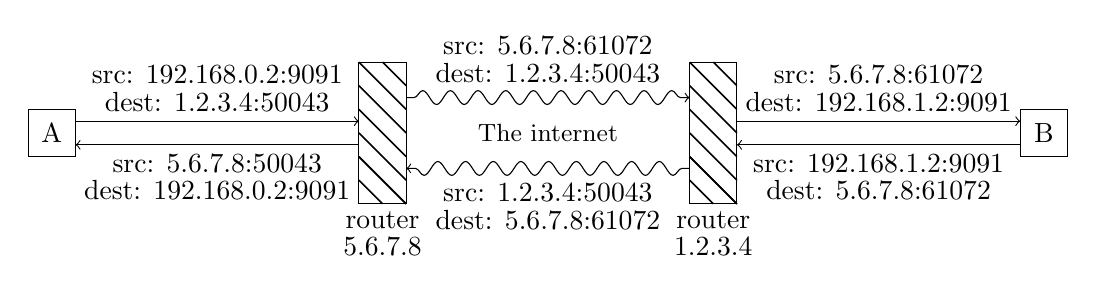
\begin{tikzpicture}
        \def\nodeWidth{0.6}
        \def\nodeHeight{0.6}
        \def\routerWidth{0.6}
        \def\routerHeight{1.8}
        \def\routerOffset{4.2}

        % Subnet A
        \draw (0,0) rectangle (\nodeWidth,\nodeHeight) node[midway] {A};

        % Interaction with router A
        \draw[->] (\nodeWidth,0.75*\nodeHeight) -- (\routerOffset,0.75*\nodeHeight) node[midway,above] {\smaller{\shortstack{src: 192.168.0.2:9091\\dest: 1.2.3.4:50043}}};

        \draw[->] (\routerOffset,0.25*\nodeHeight) -- (\nodeWidth,0.25*\nodeHeight) node[midway,below] {\smaller{\shortstack{src: 5.6.7.8:50043\\dest: 192.168.0.2:9091}}};

        % Router to router interaction
        \begin{scope}[shift={(0,-0.6)}]
            \draw[->,decorate,decoration={snake,pre length=1mm,post length=1mm}] (\routerOffset+\routerWidth,0.75*\routerHeight) -- (2*\routerOffset,0.75*\routerHeight) node[midway,above=2pt] {\smaller{\shortstack{src: 5.6.7.8:61072\\dest: 1.2.3.4:50043}}};
            \draw[->,decorate,decoration={snake,pre length=1mm,post length=1mm}] (2*\routerOffset,0.25*\routerHeight) -- (\routerOffset+\routerWidth,0.25*\routerHeight) node[midway,below=2pt] {\smaller{\shortstack{src: 1.2.3.4:50043\\dest: 5.6.7.8:61072}}};

            \path (\routerOffset+\routerWidth,0.5*\routerHeight) -- (2*\routerOffset,0.5*\routerHeight) node[midway] {\small{The internet}};
        \end{scope}

        % Subnet B
        \begin{scope}[shift={(3*\routerOffset,0)}]
            \draw (0,0) rectangle (\nodeWidth,\nodeHeight) node[midway] {B};
            % Interaction with router B
            \draw[->] (-\routerOffset+\routerWidth,0.75*\nodeHeight) -- (0,0.75*\nodeHeight) node[midway,above] {\smaller{\shortstack{src: 5.6.7.8:61072\\dest: 192.168.1.2:9091}}};

            \draw[->] (0,0.25*\nodeHeight) -- (-\routerOffset+\routerWidth,0.25*\nodeHeight) node[midway,below] {\smaller{\shortstack{src: 192.168.1.2:9091\\dest: 5.6.7.8:61072}}};
        \end{scope}

        \foreach \offset\name\address in{1/A/5.6.7.8,2/B/1.2.3.4} {
                \begin{scope}[shift={(\offset*\routerOffset,-0.6)}]
                    \def\a{0.6}
                    \def\b{1.8}
                    \def\diff{1.2}

                    \def\lw{0.2}

                    \foreach \x [count=\i] in{0,0.3,0.6,...,\a}{
                            \draw [line width=\lw mm](\x,0)--(0,\x) (\x,\b)--(\a,\b-\a+\x);
                        }
                    \foreach \x [count=\i] in{0,0.3,0.6,...,\diff}{
                            \draw [line width=\lw mm](0,\a+\x)--(\a,\x);
                        }
                    \draw (0,0) rectangle  node[below=25pt] {\smaller{\shortstack{router\\\address}}} (\routerWidth,\routerHeight);
                \end{scope}

            }
    \end{tikzpicture}
    \label{fig:successful-nat-traversal}
    \caption{Node $A$ operates in the local network 192.168.0.1/24 and listens on the canonical port 9091. $A$ is connected to a router that applies a NAT and maps $A$'s port to the dynamic port $50043$. The packet travels through the internet and arrives at the router that forwards it to $B$. $B$ is running behind a NAT as well, hence when sending a packet, $B$'s source port is mapped by the router to the dynamic port $61072$.}
\end{figure}

Hence, the crucial part is to provide the infrastructure to allow nodes to determine their public address and port, as well as a means of communication to interactively find out how to connect directly. Within the HOPR network, this is done in a decentralized way. First of all, all nodes answer STUN requests, hence nodes can find out their public address and port without relying on external resources such as public STUN servers. Secondly, nodes offer each other relay services such that connected nodes can use them as a rendezvous point to exchange connection information.

At startup, each node attempts to reserve a relay slot at several of the known relay nodes. Due to the dynamic port mapping, these nodes might be the only ones which are able to reach the node. It is therefore crucial, to preserve these connections.

Once the connections to the relay nodes have been established, the node publishes relay addresses containing the relay to which it maintains a connection.

When connecting to a new node, the initiator of the connection first fetches the direct addresses of the node and attempts to reach the destination. In case that does not work, the initiator queries the DHT to fetch relay addresses of the destination and recursively establishes a connection. Once the connection to the relay is open, the relay attempts to reach the destination. If that works, initiator and destination have a channel to exchange information. This channel is then used to transfer payload such as mixnet packets but also signalling information that might give parties the opportunity to upgrade to a direct connection using WebRTC. Once both parties found out how to connect directly, they route the traffic through the WebRTC connection. In case that is not possible, e.g. because both nodes are running behind bidirectional NATs, the relayed connection serves as fallback.

\begin{figure}[H]
    \centering
    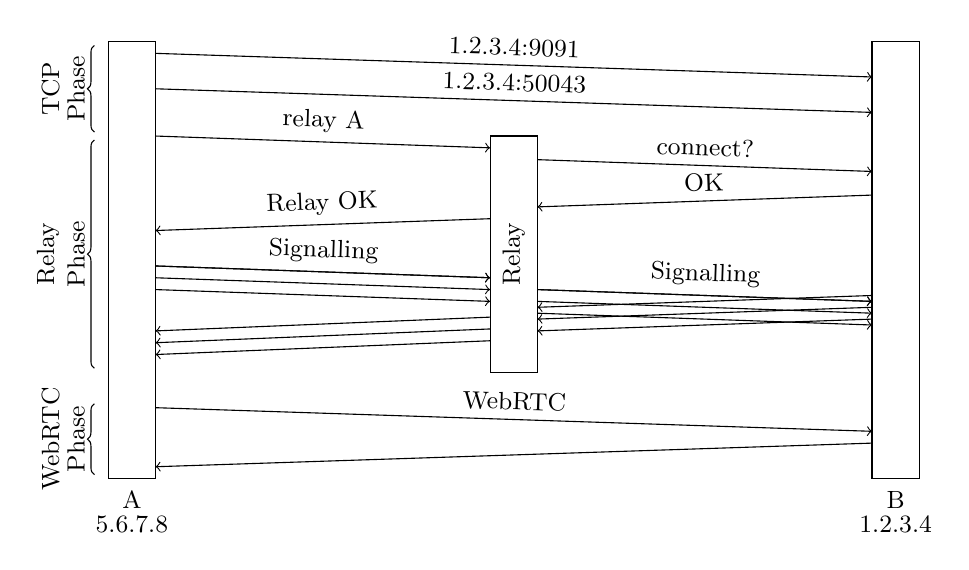
\begin{tikzpicture}
        \def\nodeHeight{5.55}
        \def\nodeWidth{0.6}
        \def\nodeOffset{4.25}
        \def\relayPhaseOffset{1.2}
        \def\webRTCOffset{4.65}
        \def\padding{0.05}

        % Nodes A and B
        \foreach \offset\name\address in{0/A/5.6.7.8,2*\nodeWidth+2*\nodeOffset/B/1.2.3.4} {
                \draw[shift={(\offset,0)}] (0,0) rectangle node[below=80pt] {\small{\shortstack{\name\\\address}}}(\nodeWidth,-\nodeHeight) ;
            }

        % Relay
        \draw (\nodeWidth+\nodeOffset,-\relayPhaseOffset) rectangle (\nodeWidth+\nodeOffset+\nodeWidth,-4.2) node[midway] {\rotatebox{90}{\small{Relay}}};

        % TCP phase
        \draw[->,shift={(0,-0.15)}] (\nodeWidth,0) -- (2*\nodeWidth+2*\nodeOffset,-0.3) node[midway,above,sloped] {\small{1.2.3.4:9091}};
        \draw[->,shift={(0,-0.6)}] (\nodeWidth,0) -- (2*\nodeWidth+2*\nodeOffset,-0.3) node[midway,above,sloped] {\small{1.2.3.4:50043}};

        \draw[decoration={brace,raise=5pt,mirror},decorate] (0,-\padding) -- node[left=5pt] {\rotatebox{90}{\small{\shortstack{TCP\\Phase}}}} (0,-\relayPhaseOffset+\padding);

        % Relay phase
        \begin{scope}[shift={(0,-\relayPhaseOffset)}]
            \draw[->] (\nodeWidth,0) -- (\nodeWidth+\nodeOffset,-0.15) node[midway,above,sloped] {
                \small{relay A}};

            \draw[->,shift={(1*\nodeWidth+\nodeOffset,-0.3)}] (\nodeWidth,0) -- (\nodeWidth+\nodeOffset,-0.15) node[midway,above,sloped] {\small{connect?}};

            \draw[->,shift={(1*\nodeWidth+\nodeOffset,-0.75)}] (\nodeWidth+\nodeOffset,0) -- (\nodeWidth,-0.15) node[midway,above,sloped] {\small{OK}};

            \draw[->] (\nodeOffset+\nodeWidth,-1.05) -- (\nodeWidth,-1.2) node[midway,above,sloped] {\small{Relay OK}};

            \foreach \i in{0,1,2} {
                    \begin{scope}[shift={(0,-1.65)}]
                        \ifnum\i=0
                            \draw[->] (\nodeWidth,0) -- (\nodeOffset+\nodeWidth,-0.15) node[midway,above,sloped] {\small{Signalling}};
                            \draw[->] (2*\nodeWidth+\nodeOffset,-0.3) -- (2*\nodeOffset+2*\nodeWidth,-0.45) node[midway,above,sloped] {\small{Signalling}};
                        \fi
                        \ifnum\i<3
                            \draw[->] (\nodeWidth,-\i*0.15) -- (\nodeOffset+\nodeWidth,-0.15-\i*0.15);
                            \draw[->] (2*\nodeWidth+\nodeOffset,-0.3-\i*0.15) -- (2*\nodeOffset+2*\nodeWidth,-0.45-\i*0.15);
                            \draw[->] (2*\nodeWidth+2*\nodeOffset,-0.375-\i*0.15) -- (\nodeOffset+2*\nodeWidth,-0.525-\i*0.15);
                            \draw[->] (\nodeWidth+\nodeOffset,-0.65-\i*0.15) -- (\nodeWidth,-0.825-\i*0.15);
                        \fi
                    \end{scope}
                }

            \draw[decoration={brace,raise=5pt,mirror},decorate] (0,-\padding) -- node[left=5pt] {\rotatebox{90}{\small{\shortstack{Relay\\Phase}}}} (0,-4.2+\relayPhaseOffset+\padding);
        \end{scope}

        % WebRTC phase
        \begin{scope}[shift={(0,-\webRTCOffset)}]
            \draw[->] (\nodeWidth,0) -- (2*\nodeWidth+2*\nodeOffset,-0.3) node[midway,above,sloped] {\small{WebRTC}};
            \draw[->] (2*\nodeWidth+2*\nodeOffset,-0.45) -- (\nodeWidth,-0.75);
            \draw[decoration={brace,raise=5pt,mirror},decorate] (0,\padding) -- node[left=5pt] {\rotatebox{90}{\small{\shortstack{WebRTC\\Phase}}}} (0,-0.9+\padding);
        \end{scope}
    \end{tikzpicture}
    \caption{$A$ intends to establish a connection to $B$. To do this, $A$ runs through three phases: \textit{TCP phase}, \textit{Relay phase} and \textit{WebRTC phase}. At first the node tries all available direct addresses. If any of them lead to a direct connection, the node is finished. Otherwise, $A$ fetches relay addresses of $B$ and connects to a relay. The relay tries to reach $B$. Once that is done, both nodes, gather information about their NAT situation and exchange with the other party. If that leads to a direct WebRTC connection, the nodes use this connection to proceed.}
\end{figure}
